\section{Dreiphasenwechselstrom und Drehfelderzeugung}
    \renewcommand{\arraystretch}{1.5}
    \begin{tabular}[b]{| C{4cm} | P{5cm} | P{9cm} |}
    	\hline
        \textbf{Sternspannungen} &
        $U_U(t) = U_m\cdot\sin\left(\omega t\right)$ \newline \newline
        $U_V(t) = U_m\cdot\sin\left(\omega t - \dfrac{2\pi}{3}\right)$ \newline \newline
        $U_W(t) = U_m\cdot\sin\left(\omega t - \dfrac{4\pi}{3}\right)$ &
        $U_U, U_V, U_W \,\widehat{=}$ den Spannungen zwischen dem Neutralleiter und dem Aussenleiter
        \\ \hline
        
        \textbf{Stern-Dreieck Umwandlung}&
        $ U_Y= \frac{U_\Delta}{3} $\newline
        $ I_Y= \frac{I_\Delta}{3} $ \newline
        $ M_Y= \frac{M_\Delta}{3} $ \newline 
        $ P_Y = \frac{P_\Delta}{3}$&
        $U = Strangspannung [V] $\newline
        $I = Strangstrom [A] $\newline
        $M = Motormoment [Nm]$ \newline 
        $P = Leistung$
        \\ \hline
                
        \textbf{Verkettete Spannung} & 	&
        $U_{UV}, U_{VW}, U_{WU}$
        \\ \hline
    \end{tabular}
    \\[0.2cm]
    \begin{minipage}[b]{\linewidth}
    	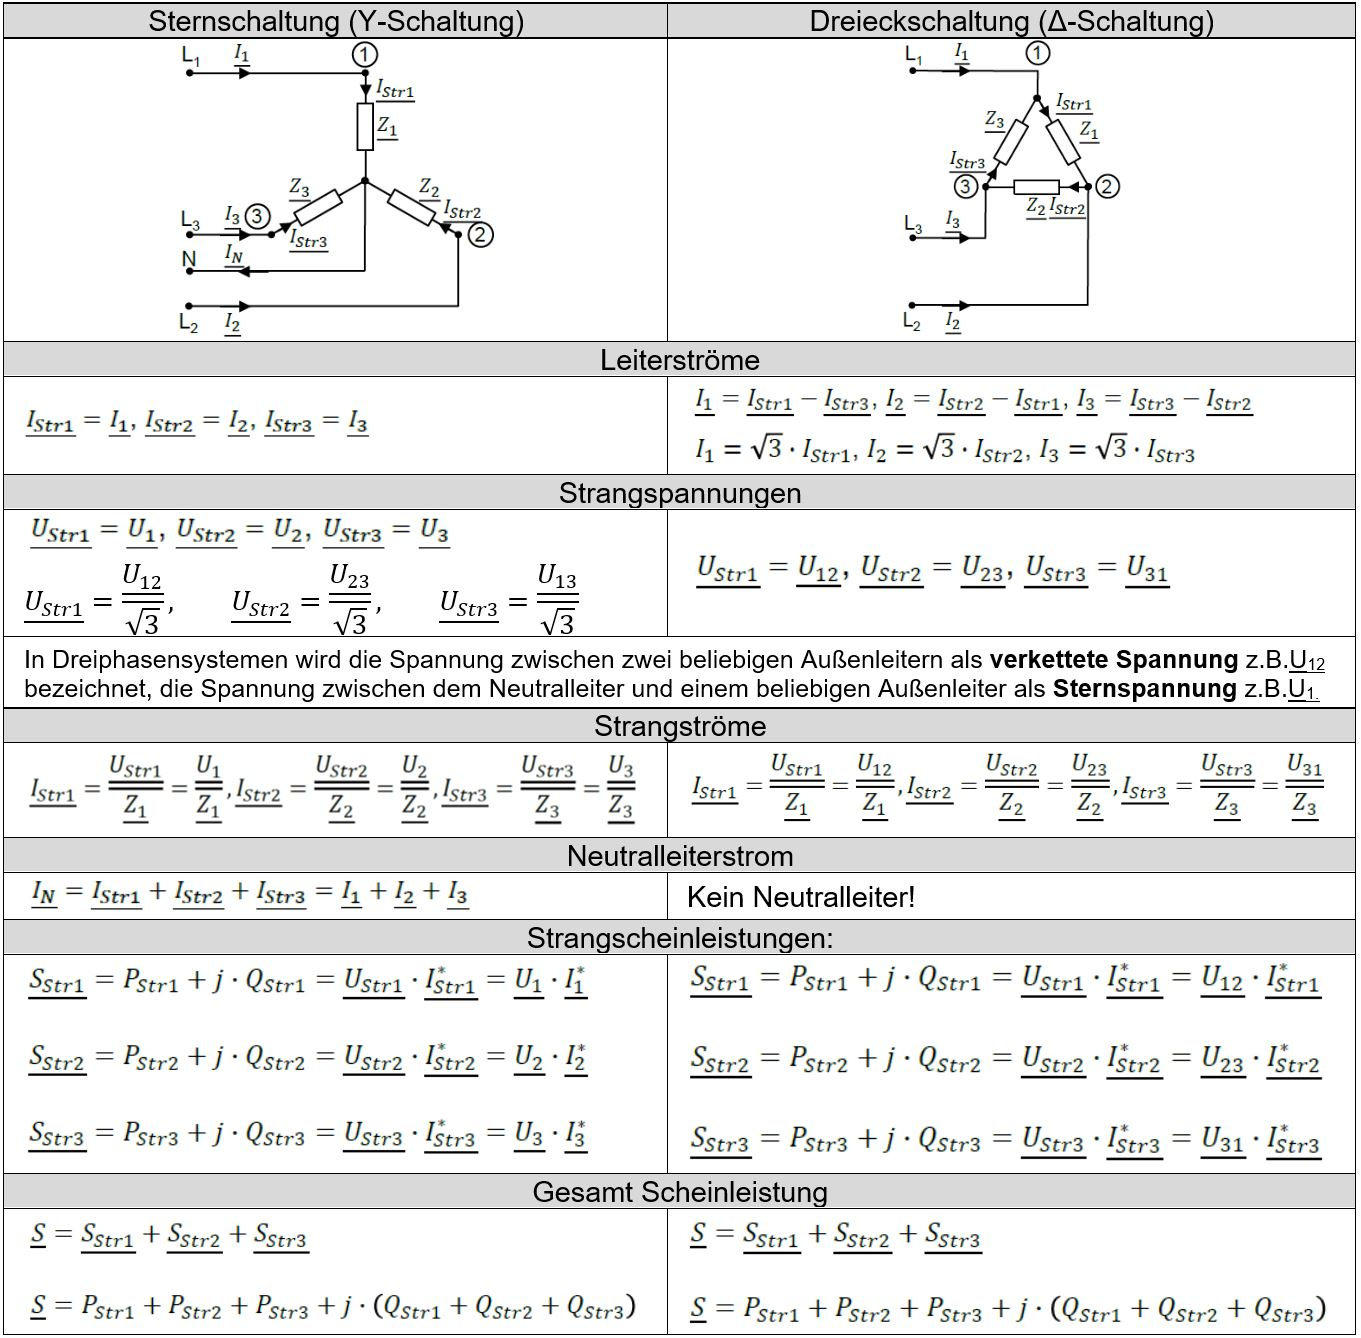
\includegraphics[scale = 0.8]{images/SternDreieck}
    \end{minipage}
    
%    \begin{minipage}[b]{0.4\linewidth}
%    	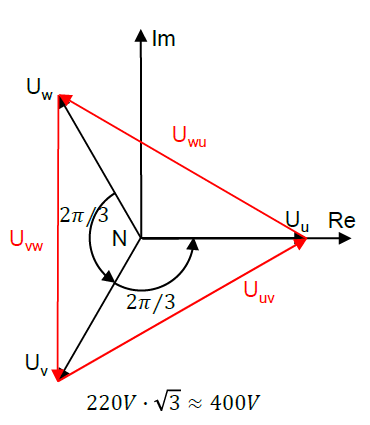
\includegraphics[width = 3.5cm]{images/Spg}
%    \end{minipage}
%    \begin{minipage}[b]{0.6\linewidth}
%    	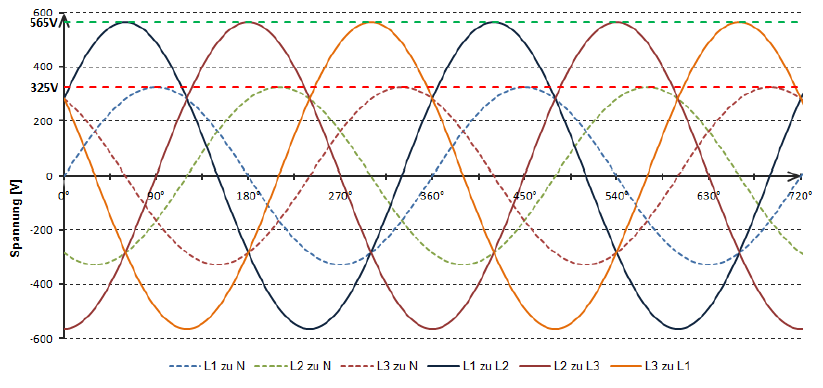
\includegraphics[width = 9cm]{images/Spg1}
%    \end{minipage}
    \clearpage
    \pagebreak
